\section{為何九七後的香港人更抗拒中國大陸?}

嚴格來說,香港人沒有在九七後立即變得更抗拒中國大陸,甚至曾有一段時間變得頗為接受。從民意調查看,香港大學從九十年代開始追蹤香港市民「對北京中央政府的信任程度」,二十多年來的數據有明顯起伏。在九十年代的初期香港社會仍然處於八九民運後的陰霾當中,對中央政府不信任的市民遠遠多於信任,數據淨值一直徘徊在負三十點。到了一九九七年末,數據回到大約零點,即信任和不信任的一樣多。數據達到最高點的時間是二零零八年初,四川地震至北京奧運前的一段時間。不過數據自此急速下跌,到了二零一二年後又回復到負數範圍。

\begin{figure}[htbp]
    \centering
    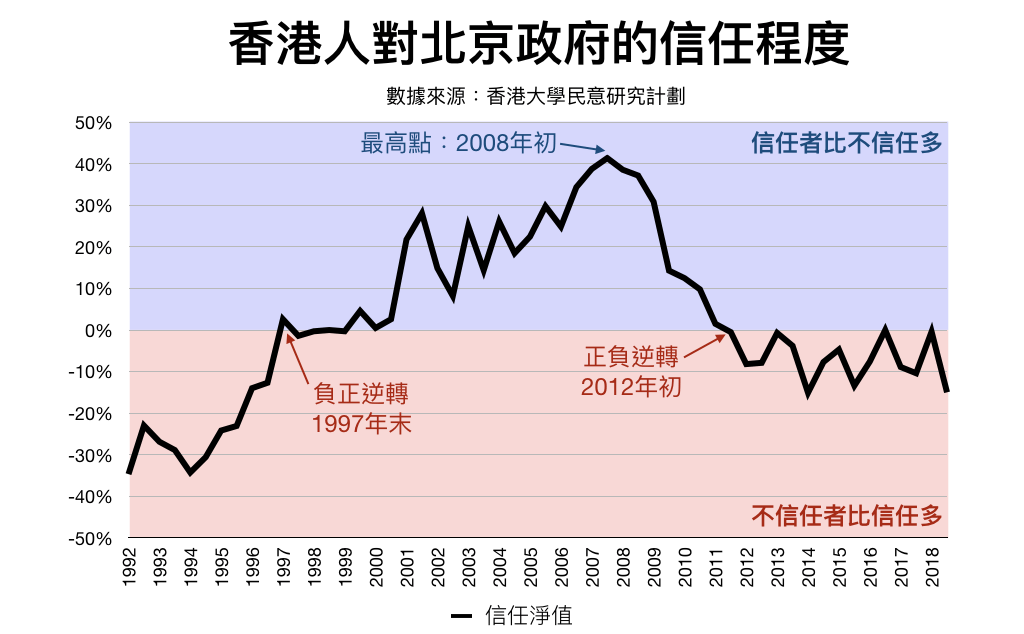
\includegraphics[width=0.7\textwidth]{c08/h-klesson1-006.png}
    \caption{香港人在1997至2008年期間曾對北京政府信任} 
\end{figure}

冰封三尺非一日之寒,香港社會在九七後對中國大陸的抗拒,和九七前的各種轉折一樣,背後同樣經歷了相當漫長的歷程。香港人對中國大陸的抗拒,可分遠因為近因去理解。近因在於中國政府近年對香港的政治操控變得明顯和直接,同時中港兩地社會交往所產生的問題又未能得到有效解決。這兩點在後面會進一步解釋。但在說近因之前,得先說明一個更廣闊的背景:中港兩地於九七後經歷了節然不同的社會發展軌跡,在價值方面形成巨大差異。價值觀落差作為遠因未必會即時爆發,但結合近因卻能製造更大的抗拒。

前文提到香港人在九七前沉醉於「明天會更好」的神話,但這夢境在特區成立的第二天便受到挑戰。泰國於一九九七年七月二日宣布放棄聯繫匯率,泰銖對美元在一天之內暴跌了百分之十七。一時之間,海外投資者紛紛警覺九十年代被吹捧的「亞洲經濟奇蹟」可能言過其實,忽視了許多東亞國家一直以來的結構性問題,大舉撤回投資做成金融緊張。國際炒家看準機會,隨即狙擊東南亞各國的貨幣謀利,並在十月份移師香港,直指香港的聯繫匯率制度。國際炒家同時在匯市和股市沽空,因為他們知道當利息水平因為幣值受壓而拉高,股票市場便會大跌,他們便可通過沽空股市獲利。這樣的雙邊操控相當成功,銀行同業隔夜拆息曾被扯高至駭人的三百厘,完全擊倒了香港股市,恆生指數由一九九七年中的接近一萬七千點,跌到一年後的不足七千點。

來到一九九八年八月,港府決定介入股市干預,國際炒家賣多少香港政府就買多少,並在八月廿八日的期指結算日創下當時史上最高的七百九十億成交紀錄,被稱為是與「國際大鱷」的「世紀大戰」。最後香港政府動用了一千二百億元儲備而險勝,成功守住股市和匯率,逼使國際炒家離開亞太地區,也減輕了人民幣貶值的壓力。然而經此一役,香港經濟已元氣大傷,對利息水平十分敏感的樓市首當其衝,然後是零售行業受打擊,失業人口於兩年內從不足八萬人升至超過二十萬,香港至七、八十年代以來的快速經濟發展迎來一個史無前例的挑戰。

回到金融危機發生之前,香港經濟本來已有不少隱憂。九七前市面對未來充滿樂觀氣氛,盲目的信心反映在樓市當中,市民對樓價上升的期望變成了一個自我實現的預言,加速樓市炒賣。與此同時,由於中方擔心港英政府於九七前賤賣土地,《中英聯合聲明》限制過渡期間每年香港土地供應不得多於五十公頃,然而這時期香港經濟快速增長,土地供應完全不能滿足需求。如是者,追蹤住宅樓價的中原城市指數由一九九六年一月的五十七點上升至一九九七年七月的一百點,短短十八個月便上升了七成多。炒賣樓宇成為極速置富的手段,甚至引來黑幫染指,每當有新建住宅樓宇開賣便會引來大批江湖小混到銷售處外排隊拿籌號,因為僅是認購籌號本身已經有炒賣價值。為求識別,不同幫派更會穿上不同顏色的風衣以作記認,變成一時都市奇觀。

當金融風暴帶來樓市爆破,很多香港人嚇然發現自從輕工業往中國大陸轉移後,香港早已出現產業空洞的問題,只是過去忙於炒賣而沒有注意到。首任特區行政長官董建華本來也想處理這個問題,並希望重構香港的經濟發展,當中以數碼港的建設最為人熟識和引起爭論。不過數碼港還未落成,美國的科網泡沫已經爆破。從一九九七開始,香港經濟一直拾級而下,經歷亞洲金融危機、科網泡沫破裂,還有美國九一一恐襲後的經濟震盪,失業率在二零零三年曾經迫近百分之八,遠遠高於九十年代平均為百分之二的水平。

然而當社會氣氛跌至前所未見的低點時,最可怕的挑戰才開始上演:非典型肺炎在二零零三年三月開始在社區爆發,世界衛生組織向香港發出旅遊警告,機場航班紛紛取消,正常經濟活動被迫中斷。在疫情初期,每天的新聞都公佈新增的染病人數,醫護人員和懷疑染病的市民都被隔離居住,市民人心惶惶。到了疫情結束,香港合共有二百九十九名市民因非典型肺炎死亡,當中包括多名醫護人員,成為香港數十年未見的嚴重災難。

更不幸的,是對抗疫情期間特區政府無法給予市民信心,反應未能乎合期望。例如儘管醫院管理局已在三月底通知衛生署疫情在社區蔓延,衛生福利及食物局局長卻仍然向公眾表示沒有擴散,並堅持學校不用停課。結果民間發動自救,家長自發拒絕讓子女上學後,政府才被迫宣告停課。面對政府回應混亂,董建華在疫情結束後曾被質疑為何沒有處分相關官員,他卻反過來批評對方膚淺,引發市民更大的不滿。

相對於主權移交前香港人自吹自擂的高峰,特區後香港政府的種種失誤無疑是落差太大。原來被捧為最專業、最有效率的香港政府,不單無法扭轉九七以來的經濟衰退,更在危機爆發時顯得手忙腳亂和措手不及。到了二零零三年,中原城市指數跌至最低的三十一點,也就是說樓價只有一九九七年時的三份之一。有些人在九七前購入物業,之後因失業而無法償還貸款,樓市大跌下又無法通過出售物業抵債,因而陷入「負資產」的困局。在這段時間,新聞常見有人抵受不住壓力而燒炭自殺,就連炭包也開始附上「珍惜生命」的字句和防止自殺熱線的電話號碼。

二零零三年是香港人難以忘懷的一年。在這一年內,一代巨星張國榮和梅艷芳以,以及著名填詞人林振強逝世,彷彿代表香港極盛輝煌的時代終於要告一段落。

非典型肺炎後的香港已經不起更多的震盪,可惜董建華卻選擇在這個時候推動《基本法》第二十三條的立法,也就是就叛國、分裂國家、煽動叛亂、顛覆中央人民政府及竊取國家機密等和國家安全相關的行為立法。面對經濟一蹶不振、失業率高企,和剛剛經歷一場重大疫症,社會普遍希望休養生息,而二十三條立法卻偏偏是一個極受爭議的議題,絕不適宜由一個民意低落和認授性存疑的政府強推。按立法程序,條例原訂於七月初於立法會表決,民間人權陣線則於七月一日特區成立紀念日舉辦「七一遊行」,結果遠超預期地有超過五十萬人上街,成為特區成立以來最大規模的群眾集會,黑壓壓的人群完全佔滿維多利亞公園和中環之間的主要街道。面對龐大的民意壓力,原來親政府的政黨也宣告改變立場,而隨著政府無法在立法會取得足夠票數通過條例,便唯有無限期押後提交審議。

h-klesson1-007.png
二十三條立法的爭議,無論對香港政府的管治、民間社會的抗爭,以至中央政府的對港政策,都是一件分水嶺事件。而對於香港身分認同本身,二十三條立法同樣帶來了微妙的改變。至特區成立首六年以來的眾多失誤,無疑把香港人本來自以為是的眾多神話打破。但與此同時,一種更實在、由下以上,強調即使窮卻不能沒有自尊的民間精神,卻慢慢逐步醞釀。

有研究指出近年香港人特別是年輕人之間越來越追求後物質價值。九七前的香港紙醉金迷,主權移交以來社會各方面卻受前所未見的挑戰,巨大的落差衝擊了許多過去視之為理所當然的社會價值,如過去主流社會認同和鼓吹的「香港社會遍佈機會」和「努力和零活變通就會發達」等說法。由此出發,再加上中港關係的改變,香港社會自二零零三年以來出現了一系列的轉化,逐漸發展成所謂的「本土思潮」,把香港身邊認同帶入一個新階段,為日後的中港矛盾埋下了種子。

傳統的需求階梯理論認為,人在追求物質安定後,才會追求非物質的目標,如自我實現和自我表達。放在公共政策來說,傾向物質主義者會強調經濟發展和城市建設,而傾向後物質主義者會較強調個人自由、環境保護和文化保育等。近年卻有研究顯示,當社會停滯不前,年輕人分享不到發展成果時,也會走向追求非物質價值。類似的趨勢似乎也在香港可見,當主權移交後經濟持續低迷,年輕人開始質疑主流價值,感到既然物質追求遙不可及,不如追尋精神上的滿足。相對於傳統的「發財立品」,現在變成「發不了財,但求有品」。

\begin{figure}[htbp]
    \centering
    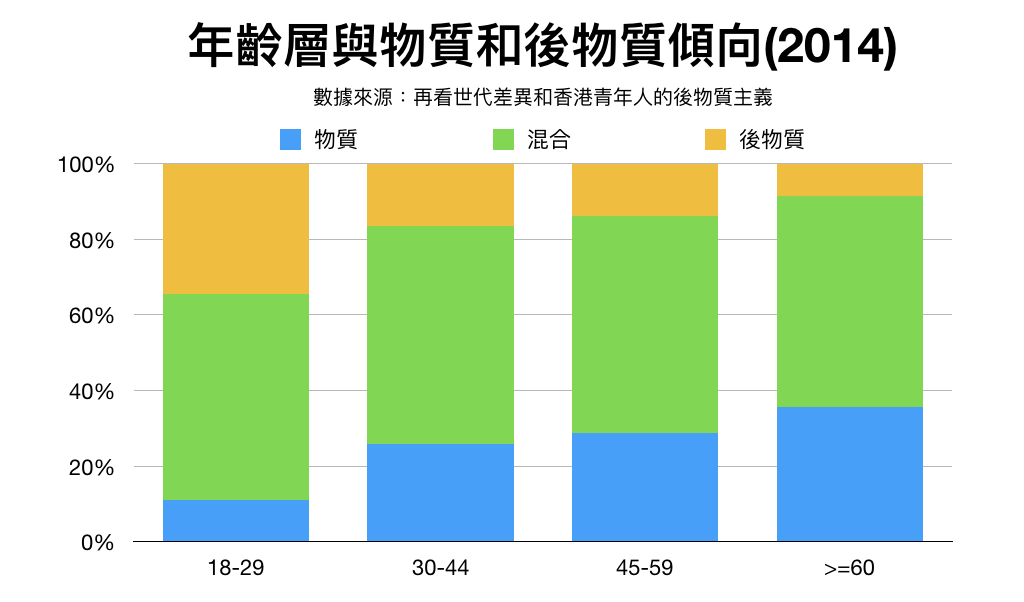
\includegraphics[width=0.7\textwidth]{c08/h-klesson1-007.png}
    \caption{香港年輕人有傾向後物質主義的趨勢} 
\end{figure}

當香港社會經歷眾多大起大跌,對大富大貴的橫財夢漸被視為虛無之際,中國大陸同時卻發生了極為不同的變化。香港經濟走到谷底的同時,中國大陸則於二零零一年底加入世界貿易組織。中國經濟除了以往低端勞動密集的出口加工業之外,也出現了國企和民企「走出去」的現象;中國不再只是外國投資的接收者,也開始帶著改革開放以來賺得的資本到世界各地。中國大陸社會如日中天的自信,與千帆過盡的香港產生巨大落差,形成新一波的身分認同之爭。

要說明香港年輕人的後物質思潮,可以二零一七年遼寧艦訪港作為案例。遼寧艦作為中國第一艘的航空母艦,對很多在中國大陸的人來說是國家發展的驕傲。而在中華民族偉大復興的宏大論述當中,晚清時期各種「喪權辱國」挫敗正是由失去海權開始,遼寧艦的建造更有其象徵意義。當遼寧艦來到香港,民間反應卻遠遠不如中國大陸熱烈。後面的原因,除了是解放軍在香港仍然會讓人想起六四鎮壓之外,就是香港社會本身對軍隊作為國家強大象徵這回事沒有多大感覺。以「船堅炮利」來量度一個國家或民族的興旺,本來就是一件很前現代的事情。放在全球治理的框架下思考,相對於成為軍事強權,一個政權是否值得尊重更在於對普世價值的追求和對人文精神的貢獻。如是者,當遼寧艦駛進維多利亞港的時候,有些香港人關注的並不是甲板上的戰機裝備,而是噴出的黑煙是否代表燃油不乎環保規定,會否污染空氣影響健康。

\begin{figure}[htbp]
    \centering
    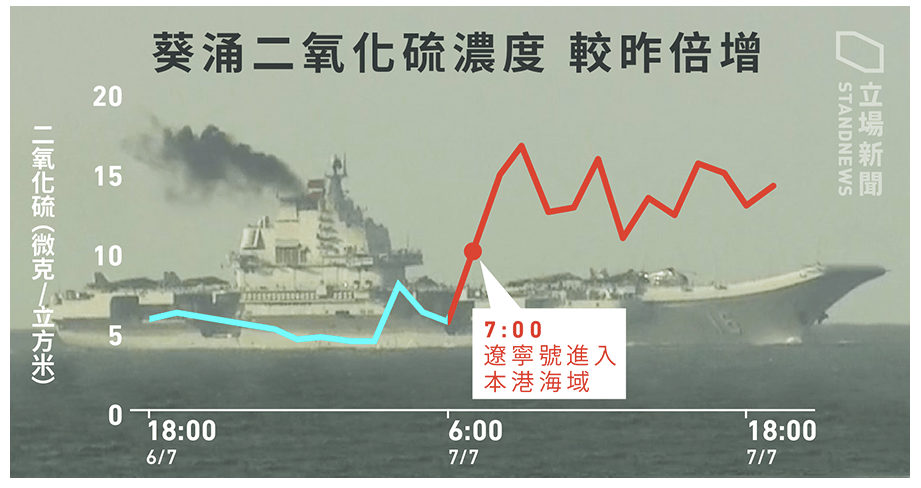
\includegraphics[width=0.7\textwidth]{c08/h-klesson1-008.png}
    \caption{香港輿論關注遼寧艦帶來空氣污染} 
\end{figure}

因為兩地所處的發展階段不一樣,中國大陸輿論有時難免會錯解香港人的反應。站在中國大陸的立場出發,很容易會以為香港近年出現對中國認同的反抗是出於兩地經濟地位對調,過去香港人習慣看不起中國大陸,現在受不了新的秩序而起。放在後物質價值的討論當中,可見這個說法如果不是錯誤解讀的話,起碼也是明顯地過度簡化。中國大陸近年的高速發展,提早二十年前已經在香港出現過;中國大陸社會在此之下的自豪感,正如前文所述,香港社會也曾經有過,而且更已反省其缺失。面對中國大陸,與其說香港人眼紅或自卑,不如說是看到過去自己在高速增長期所犯過的錯誤。

從歷史去看,中國大陸的經濟發展不能為很多香港人帶來許多認同感,在於中國大陸經濟建設本身的起點很低,而這過去的落後其實是建基於一些本來可以避免的政治動盪,香港的發展早於中國大陸正正出於香港避過了這些政治動盪。在中國大陸沒有全面反省這些政治動盪,也沒有糾正當年容許這些政治動盪發生的政治體制之前,走去慶祝這其實是遲來的經濟發展,對很多香港人來說無論在邏輯或情感上也難以說得過去。

香港的經驗也說明高速發展是特定時空的產物,總會有完結的一天,到時候社會中的深層次矛盾就會浮現。所以每當有中國大陸的意見領袖認為香港社會應放下矛盾集中精力發展經濟時,不少香港人往往會覺得可笑:香港社會早就脫離了可以通過發展經濟來舒解社會矛盾的時期,此等建議如果不是出於無知,恐怕就是為既得利益服務。香港社會已邁向後現代,中國官員的話語及其盛載的價值卻仍然停留在現代甚至是前現代(如信奉弱肉強食叢林法則,二元敵我矛盾的冷戰思維,和「發展是硬道理」代表的發展主義);當抱著這些過時思想的官員要逆向教訓邁向後現代的社會未能「與時並進」,引起強烈反彈是自然不過。這些價值觀上的明顯落差,和隨之而產生的政策失調,成為九七後香港人反而更反抗中國大陸的深層原因。而當這深層原因配上近年在政治和生活上的直接衝突,中港關係隨即急劇逆轉。


伸延閱讀:

李立峯(2016):〈再看世代差異和香港青年人的後物質主義〉,張少強、 陳嘉銘、梁啟智《香港社會文化系列》。

張少強,崔志暉(2015):《香港後工業年代的生活故事》,香港 : 三聯書店(香港)有限公司。

陳冠中(2006):〈我這一代香港人—成就與失誤〉,《我這一代香港人》,香港:牛津大學出版社。

網上資源:

\href{https://thestandnews.com/politics/遼寧號污染-葵涌二氧化硫倍升-環保署-正常波幅非偏高/}{立場報道(2017):〈葵涌二氧化硫倍升 環保署:正常波幅非偏高〉,立場新聞,2017年7月7日}